\documentclass[tikz,border=4pt]{standalone}
% Paleta y fuentes compartidas por el libro y las figuras (única fuente de verdad).
\RequirePackage{xcolor}
\definecolor{oxido}{HTML}{B7410E}
\definecolor{cobre}{HTML}{D27D2D}
\definecolor{carbon}{HTML}{2B2B2B}
\definecolor{azul}{HTML}{1F5F8B}
\definecolor{arena}{HTML}{F4EDE4}

\usepackage{fontspec}
\setsansfont{FiraSans}[Extension=.otf,UprightFont=*-Regular,BoldFont=*-SemiBold,ItalicFont=*-Italic,BoldItalicFont=*-SemiBoldItalic]
\setmonofont{FiraMono}[Extension=.otf,UprightFont=*-Regular,BoldFont=*-Medium,Scale=0.95]
\usetikzlibrary{arrows.meta,calc,positioning}
\begin{document}
\sffamily\small
\newcommand{\tit}[2]{{\bfseries\color{#1}#2}}
% Mapa del ecosistema: Rust en el centro y seis dominios alrededor.
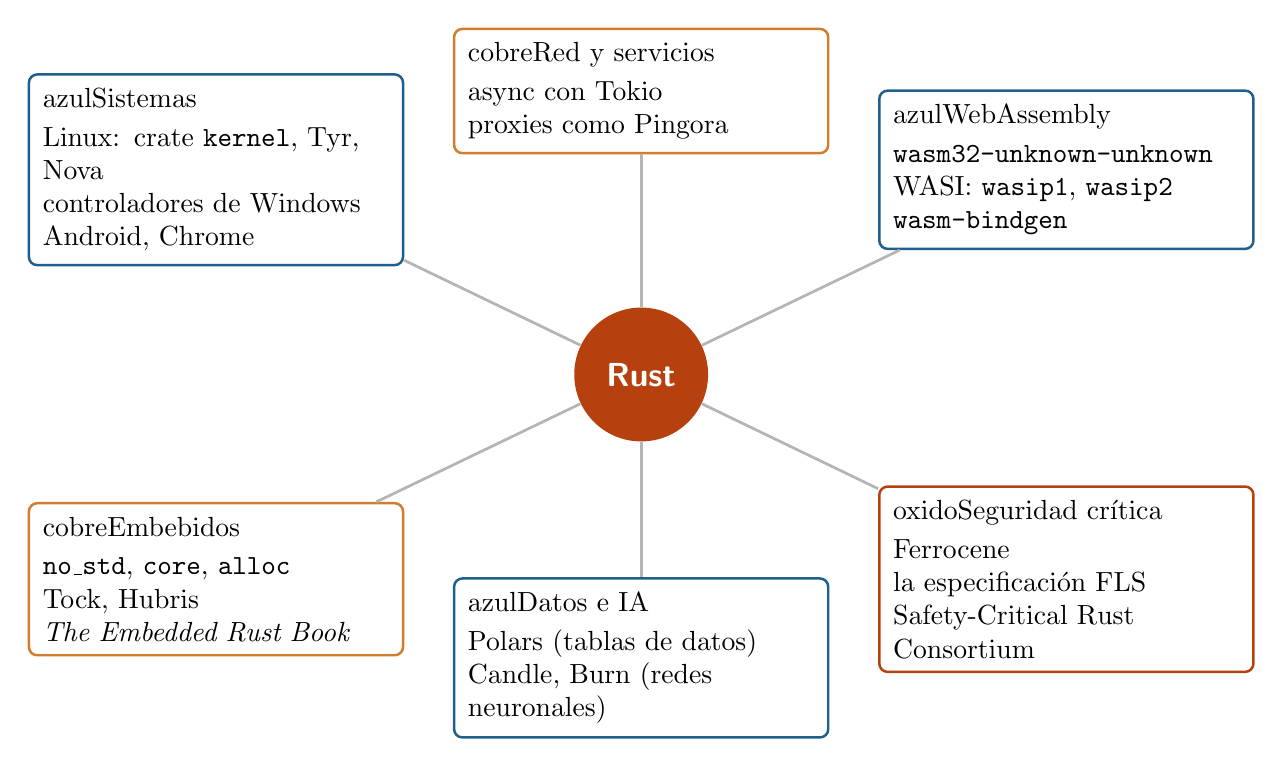
\begin{tikzpicture}[
  dominio/.style={draw=#1,line width=0.9pt,fill=white,rounded corners=3pt,
    text width=44mm,align=left,inner sep=5pt,
    execute at begin node={\hyphenpenalty=10000}},
  enlace/.style={carbon!35,line width=1pt}]
  \node[circle,fill=oxido,text=white,font=\sffamily\bfseries\large,
    minimum size=17mm] (rust) at (0,0) {Rust};
  \node[dominio=azul] (sis) at (-5.4,2.6) {%
    \tit{azul}{Sistemas}\\[2pt]
    Linux: crate \texttt{kernel}, Tyr, Nova\\
    controladores de Windows\\
    Android, Chrome};
  \node[dominio=cobre] (web) at (0,3.6) {%
    \tit{cobre}{Red y servicios}\\[2pt]
    async con Tokio\\
    proxies como Pingora};
  \node[dominio=azul] (wasm) at (5.4,2.6) {%
    \tit{azul}{WebAssembly}\\[2pt]
    \texttt{wasm32-unknown-unknown}\\
    WASI: \texttt{wasip1}, \texttt{wasip2}\\
    \texttt{wasm-bindgen}};
  \node[dominio=cobre] (emb) at (-5.4,-2.6) {%
    \tit{cobre}{Embebidos}\\[2pt]
    \texttt{no\_std}, \texttt{core}, \texttt{alloc}\\
    Tock, Hubris\\
    \emph{The Embedded Rust Book}};
  \node[dominio=azul] (ia) at (0,-3.6) {%
    \tit{azul}{Datos e IA}\\[2pt]
    Polars (tablas de datos)\\
    Candle, Burn (redes neuronales)};
  \node[dominio=oxido] (seg) at (5.4,-2.6) {%
    \tit{oxido}{Seguridad crítica}\\[2pt]
    Ferrocene\\
    la especificación FLS\\
    Safety-Critical Rust Consortium};
  \foreach \d in {sis,web,wasm,emb,ia,seg}
    \draw[enlace] (rust) -- (\d);
\end{tikzpicture}
\end{document}
